\documentclass[tikz]{standalone}
\usepackage{amsmath}
\definecolor{bgcol}{HTML}{171D2B}
\definecolor{aksen}{HTML}{F7B538}
\definecolor{biru}{HTML}{5B8DEF}
\definecolor{teks}{HTML}{FFFFFF}
\pagecolor{bgcol}
\begin{document}
% FIGUR 1: Lingkaran dibagi 16 juring, satu juring dibedakan warnanya
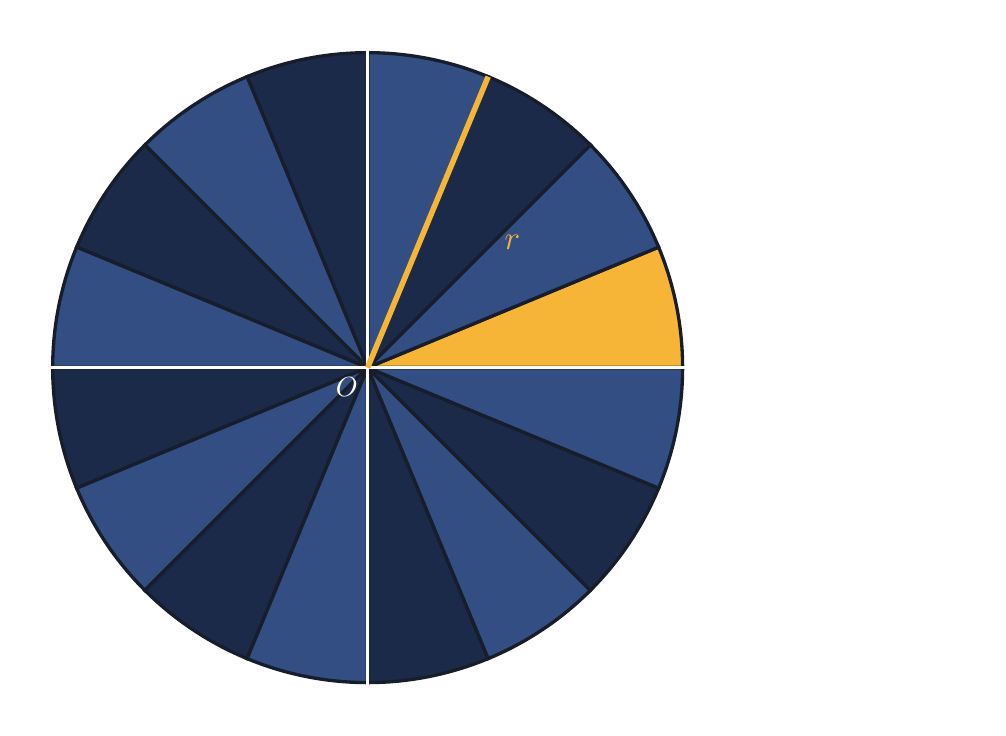
\begin{tikzpicture}[scale=1.0]
  \def\R{4}
  \def\N{16}
  \foreach \i in {0,1,...,15}{
    \pgfmathsetmacro{\a}{\i*360/\N}
    \pgfmathsetmacro{\b}{(\i+1)*360/\N}
    \ifnum\i=0
      \fill[aksen, draw=bgcol, line width=1.2pt] (0,0) -- (\a:\R) arc (\a:\b:\R) -- cycle;
    \else
      \ifodd\i
        \fill[biru!55!black, draw=bgcol, line width=1.2pt] (0,0) -- (\a:\R) arc (\a:\b:\R) -- cycle;
      \else
        \fill[biru!30!black, draw=bgcol, line width=1.2pt] (0,0) -- (\a:\R) arc (\a:\b:\R) -- cycle;
      \fi
    \fi
  }
  \draw[teks, line width=1pt] (-\R-0.3,0) -- (\R+0.3,0);
  \draw[teks, line width=1pt] (0,-\R-0.3) -- (0,\R+0.3);
  \node[teks, below left] at (0,0) {$O$};
  \node[teks, font=\large, anchor=west] at (\R+0.9,1.8) {\textbf{16 juring}};
  \node[teks, font=\large, anchor=west] at (\R+0.9,1.0) {satu dipotong,};
  \node[teks, font=\large, anchor=west] at (\R+0.9,0.2) {15 tinggal};
  \draw[aksen, line width=2pt] (0,0) -- (67.5:\R);
  \node[teks, font=\large, above left, aksen] at (33.75:\R*0.62) {$r$};
\end{tikzpicture}

% FIGUR 2: 16 juring disusun zigzag mendekati persegi panjang
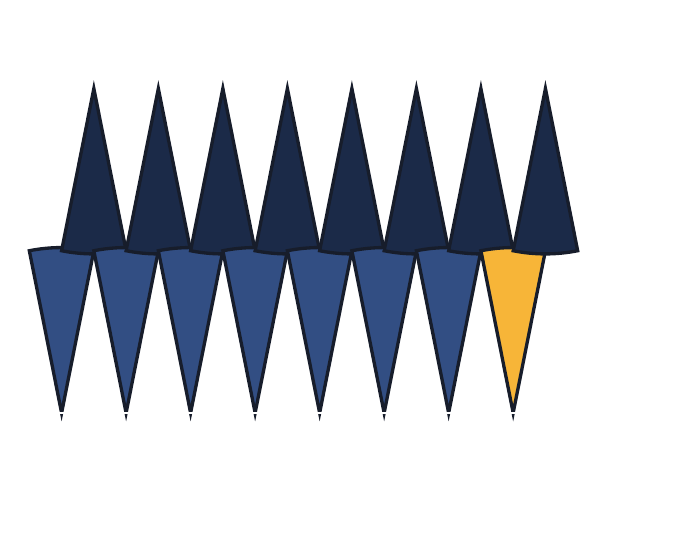
\begin{tikzpicture}[scale=1.0]
  \def\R{2.1}
  \pgfmathsetmacro{\half}{11.25}
  \pgfmathsetmacro{\s}{sin(\half)}
  \pgfmathsetmacro{\c}{cos(\half)}
  % pasangan juring: atas (biru gelap) dan bawah (biru), 8 pasang
  \foreach \k in {0,1,...,7}{
    \pgfmathsetmacro{\xu}{2*\k*\R*\s}          % puncak juring atas (di bawah)
    \pgfmathsetmacro{\xd}{(2*\k+1)*\R*\s}      % puncak juring bawah (di atas)
    % juring atas: apex di (xu,0), busur di atas
    \ifnum\k=7
      \fill[aksen, draw=bgcol, line width=1.2pt]
        (\xu,0) -- ++(90-\half:\R) arc(90-\half:90+\half:\R) -- cycle;
    \else
      \fill[biru!55!black, draw=bgcol, line width=1.2pt]
        (\xu,0) -- ++(90-\half:\R) arc(90-\half:90+\half:\R) -- cycle;
    \fi
    % juring bawah: apex di (xd, 2Rc), busur di bawah
    \fill[biru!30!black, draw=bgcol, line width=1.2pt]
      (\xd,2*\R*\c) -- ++(-90-\half:\R) arc(-90-\half:-90+\half:\R) -- cycle;
  }
  % garis dasar
  \pgfmathsetmacro{\Wtot}{16*\R*\s}
  \draw[teks, line width=0.8pt] (-0.3,0) -- (\Wtot+0.3,0);
  % dimensi lebar ~ setengah keliling
  \draw[teks, <->, line width=1pt] (0,-0.55) -- (\Wtot,-0.55)
     node[midway, below, font=\large, teks] {$\tfrac{1}{2}\cdot 2\pi r \approx \pi r$};
  % dimensi tinggi = r
  \draw[teks, <->, line width=1pt] (\Wtot+0.5,0) -- (\Wtot+0.5,\R)
     node[midway, right, font=\large, teks] {$r$};
  \node[teks, font=\normalsize, anchor=west] at (0, 2*\R*\c+0.5) {16 juring disusun berselang-seling};
\end{tikzpicture}
\end{document}
